\section{Metodologia}
\label{sec:metodologia}

A metodologia adotada neste trabalho é aplicada, experimental e orientada a reprodutibilidade. Todas as configurações de infraestrutura, código e instrumentação foram versionadas no repositório do ValorizeAI, permitindo que os experimentos de carga sejam reproduzidos de forma determinística.

\subsection{Tipo de Pesquisa e Estratégia Geral}

O estudo caracteriza-se como uma \textbf{pesquisa aplicada} conduzida sob a forma de \textbf{estudo de caso} de uma aplicação real em operação. A estratégia seguiu quatro fases iterativas:

\begin{enumerate}
    \item \textbf{Planejamento:} definição dos SLOs (latência P95~$\leq$~300~ms, taxa de erro~$<$~0,5\%, disponibilidade~$\geq$~99,5\%). Consideraram-se também as cotas do Cloud Run (10 instâncias simultâneas de 1~vCPU/1~GiB), que estabeleceram o limite teórico de throughput.

    \item \textbf{Preparação do ambiente:} módulos Terraform provisionaram a infraestrutura (VPC, Cloud Run, Cloud SQL, Redis, Cloud Tasks e balanceador). O Docker Compose reproduziu localmente PostgreSQL, Redis e ferramentas de observabilidade. O Makefile encapsulou rotinas de lint, build e execução dos cenários k6.

    \item \textbf{Execução controlada:} os cenários k6 (leitura intensiva e leitura/escrita) foram executados contra o domínio público da API, enquanto o pipeline assíncrono processava um lote adicional de tarefas enviadas ao Cloud Tasks.

    \item \textbf{Coleta e análise:} métricas de latência, throughput e taxa de erro foram extraídas dos CSVs do k6 e correlacionadas com séries temporais do Cloud Monitoring (CPU, memória, backlog de tarefas). O comportamento do pipeline assíncrono foi documentado qualitativamente e quantitativamente.
\end{enumerate}

\subsection{Arquitetura do Ambiente Experimental}

A Figura~\ref{fig:arquitetura} sintetiza o ambiente utilizado nos experimentos. O tráfego HTTP/HTTPS é roteado pelo \textbf{Cloud Load Balancer} com \textbf{Cloud CDN}, que distribui \textit{assets} estáticos e aplica políticas de segurança (WAF). A arquitetura executa três serviços Cloud Run:

\begin{itemize}
    \item \textbf{API Laravel:} responsável pelos endpoints REST exercitados nos testes.
    \item \textbf{Laravel Reverb:} servidor WebSocket dedicado, escalado independentemente.
    \item \textbf{Workers HTTP:} consumidores assíncronos acionados pelo Cloud Tasks.
\end{itemize}

O Redis (Memorystore) atua como \textit{cache} para consultas críticas e como \textit{backplane} Pub/Sub para a sincronização do Reverb. O banco transacional permanece no \textbf{Cloud SQL for PostgreSQL}, configurado como instância de 2~vCPU e 16~GiB de RAM para refletir o ambiente produtivo. O \textbf{Cloud Tasks} executa o pipeline assíncrono por meio de requisições \textit{push}, permitindo escalabilidade automática dos workers. O \textbf{Cloud Storage} integra o sistema, mas não foi exercitado nos testes.

\subsection{Desenvolvimento da Aplicação e Modelo de Dados}

O backend Laravel concentra o domínio financeiro e expõe APIs consumidas pelo front-end em React. Os workers HTTP processam tarefas intensivas, como importações de extratos, geração de relatórios e envio de notificações. O modelo relacional multi-inquilino, mostrado na Figura~\ref{fig:modelo-dados}, organiza usuários, contas, transações, categorias, orçamentos e embeddings vetoriais, permitindo cenários realistas durante os testes.

\subsection{Ferramentas e Processo de Preparação}

A reprodutibilidade foi garantida por três pilares:

\begin{itemize}
    \item \textbf{Infraestrutura como Código (IaC):} cada componente (Cloud SQL, Redis, Cloud Run, Tasks e balanceador) possui módulo Terraform independente. Outputs conectam automaticamente credenciais, redes e endpoints entre serviços, evitando divergências.

    \item \textbf{Ambientes determinísticos:} Docker Compose e Makefile garantem que a aplicação seja testada sempre com a mesma versão do stack (PHP 8.4, PostgreSQL, Redis), evitando variabilidade entre execuções.

    \item \textbf{Observabilidade:} métricas de CPU, fila, memória e latência foram coletadas no Cloud Monitoring. Logs e traces complementaram a identificação dos pontos de saturação.
\end{itemize}

\subsection{Planejamento dos SLOs e Desenho dos Cenários}

Com base na literatura de SRE \cite{mccoy_slo_2020,google_sre_book_main}, adotaram-se três metas: latência P95 $\leq 300$~ms, erro $<$0{,}5\% e disponibilidade $\geq$99,5\%. As cotas do Cloud Run definiram o limite físico dos experimentos (10 instâncias de 1~vCPU). Os testes foram projetados para atingir e analisar o comportamento nessa zona de saturação.

Foram definidos três experimentos:

\begin{enumerate}
    \item \textbf{Cenário de leitura intensiva:} 1.000 VUs acessando o endpoint \texttt{GET /api/transactions} durante 17 minutos. O roteiro alternou contas, filtros e um \textit{think time} de 1~s para simular interação real.

    \item \textbf{Cenário misto leitura/escrita:} 650 VUs alternando entre consultas e criação de transações (65\% leitura, 20\% escrita, 15\% contas). Esse fluxo replica a proporção observada nos logs reais.

    \item \textbf{Teste assíncrono:} publicação de 51.580 tarefas no Cloud Tasks, monitorando o tempo de drenagem e o pico de instâncias dos workers.
\end{enumerate}

Os cenários foram estruturados com ramp-ups progressivos (150 $\rightarrow$ 1.000 VUs) para aquecer o cache e observar o comportamento nas proximidades do teto de instâncias.

\subsection{Execução dos Experimentos}

Cada rodada seguiu o protocolo:

\begin{enumerate}
    \item \textbf{Preparação dos dados:} povoamento do PostgreSQL com seeds e factories, e pré-aquecimento do Redis.
    \item \textbf{Disparo dos cenários k6:} execução automatizada via Makefile, registrando SLIs e eventos relevantes.
    \item \textbf{Coleta automática:} exportação dos resultados do k6 para CSV (latência, erros, uso de VUs).
    \item \textbf{Teste de filas:} disparo massivo de tarefas e monitoramento do backlog no Cloud Tasks.
\end{enumerate}

\subsection{Coleta e Integração das Evidências}

As evidências utilizadas na análise incluem:

\begin{itemize}
    \item \textbf{Tabelas e séries de latência/throughput} extraídas do k6;
    \item \textbf{Métricas de infraestrutura} (CPU, instâncias ativas, backlog da fila);
    \item \textbf{Logs e observações experimentais}, destacando comportamentos de saturação.
\end{itemize}

Essa abordagem garante rastreabilidade completa entre arquitetura, ambiente, experimentos e resultados, pois todos os artefatos , código, infraestrutura e cenários , estão versionados no repositório.

\begin{figure}[ht]
    \centering
    \resizebox{\linewidth}{!}{%
    \begin{tikzpicture}[node distance=1.5cm, every node/.style={font=\footnotesize, align=center}]
        \node (cdn) [draw, rounded corners, fill=gray!15, minimum width=5cm, minimum height=0.9cm] {Cloud Load Balancer + Cloud CDN};
        \node (api) [draw, rounded corners, fill=blue!10, minimum width=3cm, minimum height=0.9cm, below left=1.1cm and 2.0cm of cdn] {Cloud Run\\API};
        \node (reverb) [draw, rounded corners, fill=blue!10, minimum width=3cm, minimum height=0.9cm, below=1.1cm of cdn] {Cloud Run\\Reverb};
        \node (workers) [draw, rounded corners, fill=blue!10, minimum width=3cm, minimum height=0.9cm, below right=1.1cm and 2.0cm of cdn] {Cloud Run\\Workers};
        \node (shared) [draw, rounded corners, fill=orange!15, minimum width=6cm, minimum height=1.2cm, below=1.3cm of reverb] {Cloud SQL + Memorystore (Redis) + Cloud Storage};
        \node (tasks) [draw, rounded corners, fill=green!10, minimum width=5cm, minimum height=0.9cm, below=1.0cm of shared] {Cloud Tasks};

        \draw[->, thick] (cdn) -- (api);
        \draw[->, thick] (cdn) -- (reverb);
        \draw[->, thick] (cdn) -- (workers);
        \draw[->, thick] (api) -- (shared);
        \draw[->, thick] (reverb) -- (shared);
        \draw[->, thick] (workers) -- (shared);
        \draw[->, thick] (api) |- (tasks);
        \draw[->, thick] (tasks) -| (workers);
    \end{tikzpicture}}
    \caption{Arquitetura utilizada nos experimentos.}
    \label{fig:arquitetura}
\end{figure}

\begin{figure}[ht]
    \centering
    \resizebox{0.95\linewidth}{!}{%
    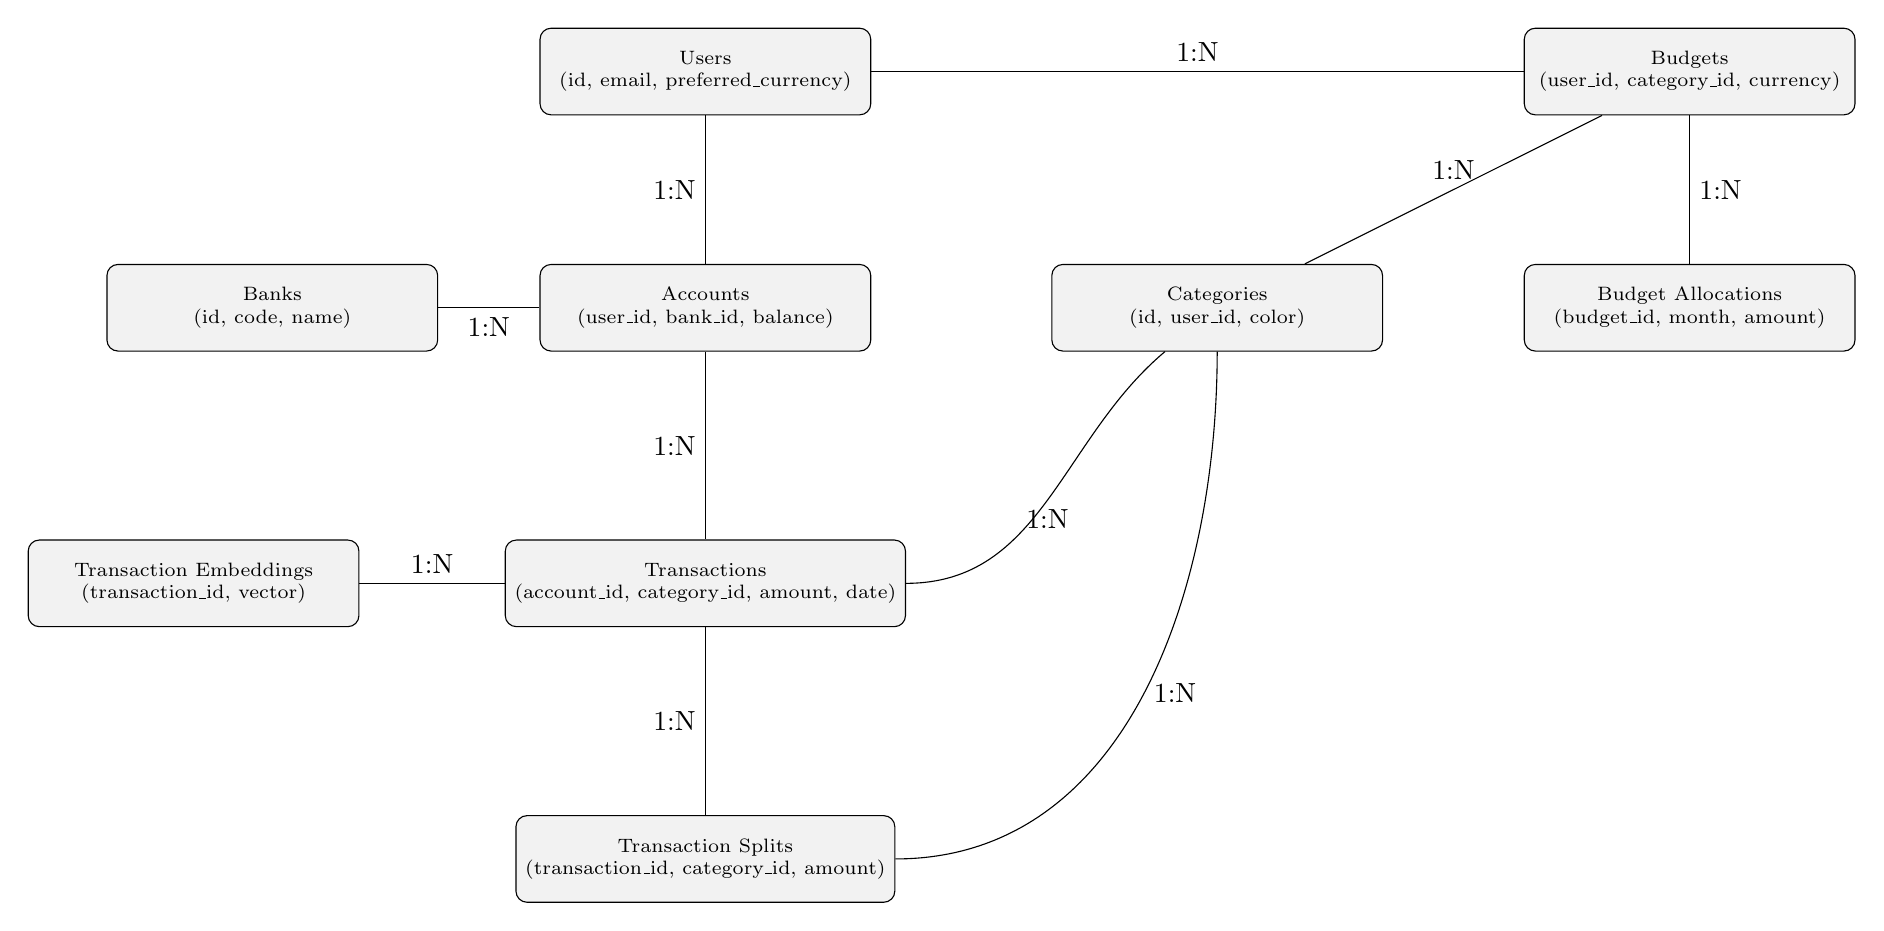
\begin{tikzpicture}[
        table/.style={draw, rounded corners, fill=gray!10, minimum width=4.2cm, minimum height=1.1cm, font=\scriptsize, align=center},
        every edge/.style={->, very thick, >=Stealth}
    ]
        \node (users) at (0,1.5) [table] {Users\\(id, email, preferred\_currency)};
        \node (banks) at (-5.5,-1.5) [table] {Banks\\(id, code, name)};
        \node (accounts) at (0,-1.5) [table] {Accounts\\(user\_id, bank\_id, balance)};
        \node (transactions) at (0,-5.0) [table] {Transactions\\(account\_id, category\_id, amount, date)};
        \node (splits) at (0,-8.5) [table] {Transaction Splits\\(transaction\_id, category\_id, amount)};

        \node (categories) at (6.5,-1.5) [table] {Categories\\(id, user\_id, color)};
        \node (embeddings) at (-6.5,-5.0) [table] {Transaction Embeddings\\(transaction\_id, vector)};
        \node (budgets) at (12.5,1.5) [table] {Budgets\\(user\_id, category\_id, currency)};
        \node (allocations) at (12.5,-1.5) [table] {Budget Allocations\\(budget\_id, month, amount)};

        \draw (users) -- node[midway,left]{1:N} (accounts);
        \draw (banks) -- node[midway,below]{1:N} (accounts);
        \draw (accounts) -- node[midway,left]{1:N} (transactions);
        \draw (transactions) -- node[midway,left]{1:N} (splits);
        \draw (transactions) -- node[midway,above]{1:N} (embeddings);

        \draw (users) -- node[midway,above]{1:N} (budgets);
        \draw (categories) -- node[midway,above]{1:N} (budgets);
        \draw (budgets) -- node[midway,right]{1:N} (allocations);

        \draw (categories) to[out=-140,in=0] node[midway,below]{1:N} (transactions);
        \draw (categories) to[out=-90,in=0] node[midway,right]{1:N} (splits);
    \end{tikzpicture}}
    \caption{Modelo lógico central derivado do esquema relacional do ValorizeAI.}
    \label{fig:modelo-dados}
\end{figure}



